% Roadmap figure from the MATH 556 notes (front matter). Compile with the notes preamble.
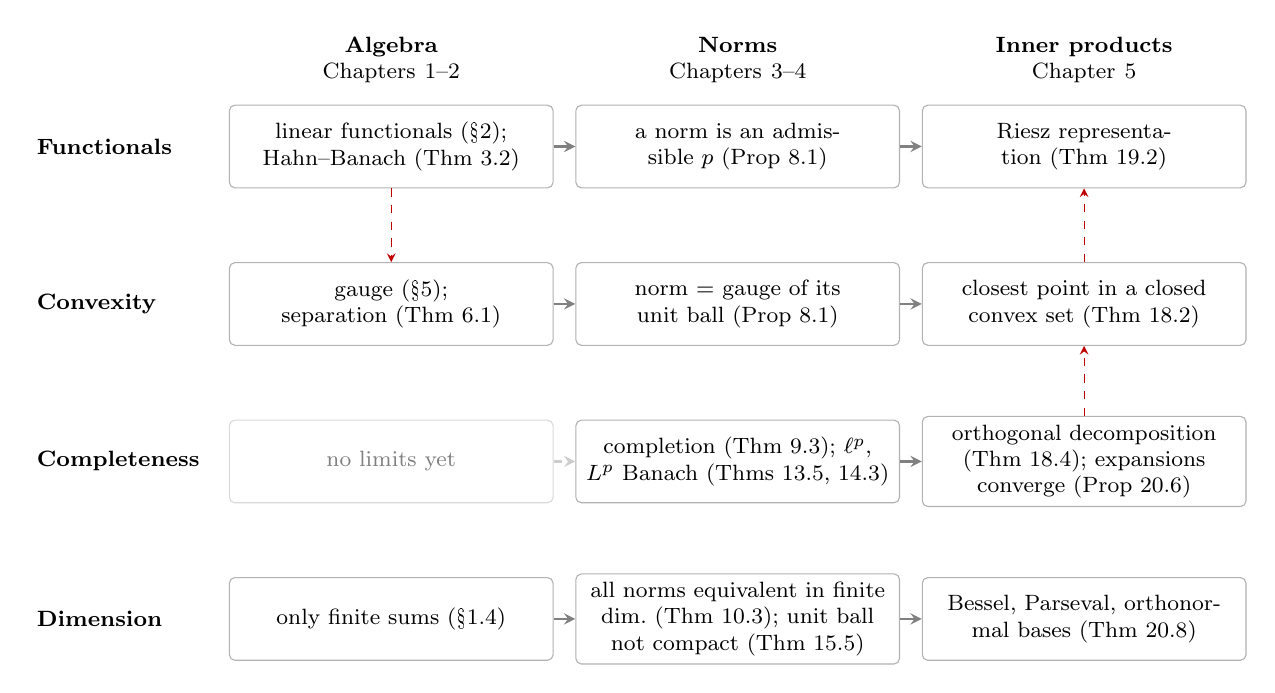
\begin{tikzpicture}[>=stealth, x=1cm, y=1cm,
    box/.style={draw=gray!60, rounded corners=2pt, fill=white, text width=3.9cm, align=center, font=\footnotesize, inner sep=3pt, minimum height=1.05cm},
    lab/.style={font=\footnotesize\bfseries, text width=2.4cm, align=left},
    hd/.style={font=\footnotesize\bfseries, align=center, text width=3.9cm}]
    \node[hd] at (3.3,1.1) {Algebra\\ \normalfont Chapters 1--2};
    \node[hd] at (7.7,1.1) {Norms\\ \normalfont Chapters 3--4};
    \node[hd] at (12.1,1.1) {Inner products\\ \normalfont Chapter 5};
    % functionals
    \node[lab] at (0,0) {Functionals};
    \node[box] (f1) at (3.3,0) {linear functionals (\S2);\\ Hahn--Banach (Thm~3.2)};
    \node[box] (f2) at (7.7,0) {a norm is an admissible $p$ (Prop~8.1)};
    \node[box] (f3) at (12.1,0) {Riesz representation (Thm~19.2)};
    % convexity
    \node[lab] at (0,-2.0) {Convexity};
    \node[box] (c1) at (3.3,-2.0) {gauge (\S5);\\ separation (Thm~6.1)};
    \node[box] (c2) at (7.7,-2.0) {norm $=$ gauge of its unit ball (Prop~8.1)};
    \node[box] (c3) at (12.1,-2.0) {closest point in a closed convex set (Thm~18.2)};
    % completeness
    \node[lab] at (0,-4.0) {Completeness};
    \node[box, draw=gray!30, text=gray] (k1) at (3.3,-4.0) {no limits yet};
    \node[box] (k2) at (7.7,-4.0) {completion (Thm~9.3); $\ell^p$, $L^p$ Banach (Thms~13.5, 14.3)};
    \node[box] (k3) at (12.1,-4.0) {orthogonal decomposition (Thm~18.4); expansions converge (Prop~20.6)};
    % dimension
    \node[lab] at (0,-6.0) {Dimension};
    \node[box] (d1) at (3.3,-6.0) {only finite sums (\S1.4)};
    \node[box] (d2) at (7.7,-6.0) {all norms equivalent in finite dim.\ (Thm~10.3); unit ball not compact (Thm~15.5)};
    \node[box] (d3) at (12.1,-6.0) {Bessel, Parseval, orthonormal bases (Thm~20.8)};
    % arrows along threads
    \foreach \a/\b in {f1/f2, f2/f3, c1/c2, c2/c3, k2/k3, d1/d2, d2/d3} \draw[->, thick, gray] (\a) -- (\b);
    \draw[->, thick, gray!40, dashed] (k1) -- (k2);
    % meeting points
    \draw[->, red!75!black, dashed] (f1) -- (c1);
    \draw[->, red!75!black, dashed] (k3) -- (c3);
    \draw[->, red!75!black, dashed] (c3) -- (f3);
\end{tikzpicture}
